\chapter{Methods}

\section{\dBG{s}}
\label{sec:dBG}

% - Detailed explanation of \dBG of a set of DNA sequences
%   - reverse complements
% - How it is going to be used
% - Operations
%   - Insert node
%   - Insert edge
%   - Query node
%   - Query edge / star 
% - Space-efficient representations - that's what we propose

The \keyterm{\dBG of order $k$} of a string \strdef{x}{n}, $G(X;k)=(V,E)$, is defined as the directed graph whose nodes $V$ represent all distinct \kmer{s} (i.e. substrings of length $k$) of \strname{X}, and such that any two nodes representing $(k-1)$-overlapping \kmer{s} are connected by an edge labeled by the last character of the second \kmer. For example if $k=3$ and $X$ contains the substring \chr{ACGT} then the consecutive triplets \chr{ACG} and \chr{CGT} will originate the edge $\chr{ACG}\stackrel{\chr{C}}{\longrightarrow}\chr{CGT}$. Hence the edges $E$ represent all distinct $(k+1)$-mers of $X$. 
% That is, given two nodes on the graph, they each represent a distinct sequence of symbols $S_1$ and $S_2$, and there is an edge between them if and only if the tail of $S_1$ is the head of $S_2$.

In genome sequencing, \dB graphs are used in the assembly process to represent the distinct \kmer{s} in a set \readset of randomly distributed fragments of the source DNA \strname{S}, called \keyterm{reads}, generated by the sequencing machines. The number of reads generated ($|\readset|$) is determined by the \keyterm{coverage} of the sequencing process: the number of times \strname{S} was cloned and sequenced. Ideally, \strname{S} could be obtained from an Eulerian traversal of $G(\readset, k)$. Unfortunately however, due to sequencing errors and repeats, such a straightforward approach is not feasible, but the \dBG can still be used to produce a collection of partial assemblies, called \keyterm{contigs}, which can then be further combined to form the original genome \cite{Pevzner2001}. Figure~\ref{fig:dbgexample} presents an example of the \dBG in this context.

\begin{figure}[htbp]
	\begin{center}
    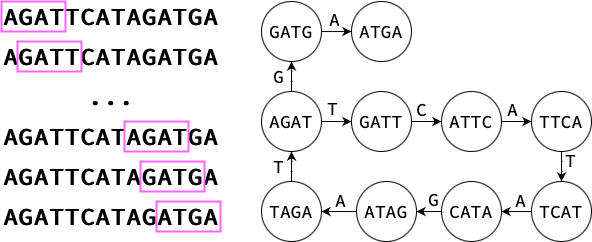
\includegraphics[width=0.8\textwidth]{figures/dbg-example}
	\end{center}
	\caption{Example of a \dBG. $k=4$}\label{fig:dbgexample}
\end{figure}

\subsection{Reverse Complements}
\label{subsec:dBG-reversecomplements}

One difficulty of using \dBG to represent DNA data is the presence of \keyterm{reverse complements}. When generating sequencing reads, the machine reads either of the two complementary strands of a fragment of the input DNA. That is, the output read may correspond to the sequence \strname{S} in the forward (5'-3') direction, or its reverse complement \strname{\overline{S}} in the backward (3'-5') direction, with
\strname{\overline{S}} being obtained from \strname{S} by swapping each base with its Watson-Crick complement
($\A \leftrightarrow \T$, $\C \leftrightarrow \G$) and then reversing the string, and vice versa. 

To deal with reverse complements, reads are processed twice\asq{can be made active? ``we'' doesn't apply as we're talking in abstract}, once in each direction. Nodes representing \kmer{s} that are reverse complements of each other can then be merged, with edges made bi-directed. Alternatively, those nodes can be kept distinct, resulting in a symmetric graph in which, as noted by Conway \& Bromage, ``a forward traversal corresponds to the backwards traversal on the reverse complement path, and vice versa.'' \cite{Conway2011}
% As in \cite{Conway2011}, this will be treated by processing
% all reads in both directions, without, however, merging nodes representing reverse complements. As noted by Conway \& Bromage: ``This
% makes the graph symmetric; a forward traversal corresponds to a backwards traversal on the reverse complement path, and vice versa.``
% \cite{Conway2011}

\subsection{Selecting the \kmer{s} for the \dBG}
\label{subsec:dBG-selectingkmers}

Another difficulty of using a \dBG to represent DNA data is dealing with sequencing errors. During the sequencing process, there is a small error rate associated with reading any base from \strname{S} (0.1\%--1\% per base in Illumina \cite{Metzker2010}). As a result, many of the \kmer{s} extracted from the reads in \readset are erroneous: As discussed by Conway \& Bromage, this causes the number of spurious \kmer{s} to grow proportionally to the number of bases in the reads ($\sum_{\strname{X}_i \in \readset} |\strname{X}_i|$), determined by the coverage, while the number of true \kmer{s} is proportional to the size of the genome ($|\strname{S}|$) \cite{Conway2011}.

Although modern sequencing machines generate a quality score associated with each base read, it is not possible to exactly determine what parts of the read are erroneous and what parts are correct. As such, it is impossible to exactly determine if a \kmer should be added to the \dBG without more information. Because the original DNA is sequenced a number of times equal to the coverage $c$, real \kmer{s} are expected to appear a number of times close to $c$ (or a multiple of $c$ in case of repeats). Spurious \kmer{s} resulting from sequencing errors, however, don't benefit from this fact and are commonly low-frequency or even unique \cite{Conway2011} \cite{Zhang2014} \cite{Ghosh2019}. As such, a natural way of filtering the \kmer{s} obtained from the reads is to discard those that have a low frequency. I.e. a \kmer $X$ obtained from the reads is considered to be a real \kmer iff it occurs more than some threshold $t$, being added to the \dBG.

Counting \kmer{s} in a set of reads in a time- and space-efficient manner is, in itself, a challenging task, and many methods exist to achieve this, each with their own set of functionalities and trade-offs. It is also commonly performed as a standalone step separate from \dBG construction \cite{Zhang2014}. Some assemblers, however, introduce \kmer counting as a part of the \dBG construction, such as the \emph{FastEtch} assembler, which uses a \cm sketch (discussed in Section~\ref{sec:countmin}) to count the \kmer{s} during \dBG construction \cite{Ghosh2019}.

\asq{Discussion about false negatives arising from choice of $t$? None of the articles I've read talk about the fact that some real \kmer{s} might not be represented in the \dBG, so I wouldn't really know what to put here as I don't have a firm grasp on how false negative rates impact assembly.}

\subsection{\dBG representation}
\label{subsec:dBG-representation}

A \dBG can be represented either by its set of nodes (\kmer{s}) or edges ($(k+1)$-mers) equivalently, as one can be derived from the other. Therefore, a structure that can determine if a given node $x$ is a member of $G$ can represent the \dBG. Conway \& Bromage showed that the lower bound on the space required to \emph{exactly} represent these \keyterm{membership data structures} (MDS's) is $\Omega(n \log n)$, with $n=|V(G)|$ \cite{Conway2011}.

In order to further improve space-efficiency, new representations were created that trade deterministic exactness for a probabilistic approach. Pel \emph{et al.} showed that a probabilistic representation based on a Bloom Filter \asq{citation needed?} could accuratly represent a \dBG with as little as 4 bits per \kmer \cite{Pell2012}. \toconsider{They also showed that false positive rates could be as high as $15\%$ before false connectivity began to dominate the graph structure.}

However, Bowe \emph{et al.} \cite{Bowe2012} and Chikhi \& Rizk \cite{Chikhi2013} independently observed that giving up deterministic exactness isn't the only option for obtaining better space-efficiency, introducing two new representations that use $O(n)$ and $O(n \log k)$ bits, respectively, and allow for an exact traversal of the \dBG from a starting set of known member nodes. This is possible due to the fact that a \dBG is not queried for membership of random nodes, but rather for potential neighbors of nodes already known to be in the graph. As such, the structures designed by the two groups do not offer a deterministically exact membership query operation, instead offering a neighborhood query operation that is exact for the members of the graph \cite{Bowe2012} \cite{Chikhi2013}. Chikhi \emph{et al.} later named this new form of representation a \keyterm{Navigational Data Structure} (NDS) and showed that the lower bound on the number of bits required to exactly represent a \dBG with an NDS is $3.24n$ \cite{Chikhi2014}.

Beyond the distinction between probabilistic and exact, and MDSs and NDSs, there is also a distinction between \keyterm{static} and \keyterm{dynamic} representations for \dBG. Static representations are constructed once and never altered, whereas dynamic representations support operations such as insertion and deletion of nodes, useful in population-scale studies due to their everchanging nature \cite{Alipanahi2021}.

% A \dBG can be represented either by its set of nodes (\kmers) or edges ($(k+1)$-mers) equivalently, as one can be derived from the other.
% As such, a structure that can answer queries about the presence of a given node on the graph is enough to
% represent the graph. Conway\&Bromage showed that the lower bound on the space required to
% \emph{exactly} represent a \dBG is $\Omega(n \log n)$ bits, where $n$ is the number of nodes\remove[isn't this obvious?]{,
% and $4^k > n$}\cite{Conway2011}.

% \asq{Isso precisa ser reescrito: NDSs não são necessariamente representações probabilisticas. Elas apenas substituem a consulta de presença de um nó pela consulta de vizinhança.}

% In order to further improve space-efficiency, new representations were created that trade deterministic exactness for a probabilistic approach. For instance, the so-called \keyterm{Navigational Data Structures} (NDS) have some probability of giving an erroneous answer to a membership query, 
% but can still be used to navigate the graph \cite{Chikhi2014}. This \change{definition is useful}{is} due to the fact that a \dBG is usually not queried for membership of \change{randomly selected}{random} nodes, but rather \remove{only} potential neighbors of \change{a known member node is queried}{nodes already known to be in the graph}. In the same paper where they introduce
% the idea of NDS \cite{Chikhi2014}\paguso{correct?}\asq{Esse artigo de Chikhi \emph{et al.} é a introdução e formalização do conceito de NDSs em oposição às Membership Data Structures. Em segunda leitura, porém, categorizar nossas estruturas como NDSs é incorreto porque NDSs devem dar respostas exatas para consultas de vizinhança, o que nós não garantimos.}, Chikhi \emph{et al.} also present a lower bound for the number of bits needed to represent such a structure as $3.24n$.
% In sections \ref{sec:debruijncountmin} and \ref{sec:debruijnhashtable} we will introduce two new NDS's. \asq{É necessário reiterar
% os objetivos das duas estrutas aqui, visto que isso já seria feito na introdução e é feito nas próprias sessões dedicadas a cada estrutura?}\paguso{até o momento, acho que não.}

\subsubsection{Operations}
\label{subsubsec:dbg-operations}

Chikhi \emph{et al.} \cite{Chikhi2019} present the following set of operations common to many data structures for representing a \dBG \asq{Na verdade, eles falam especificamente de "set of \kmer{s}". Sendo que, no final das contas, um \dBG não deixa de ser um "set of \kmer{s}"}.

\begin{enumerate}
  \item \emph{Construction} of the data structure
  \item \emph{Insertion} of a new \kmer
  \item \emph{Deletion} of an existing \kmer.
  \item \emph{Membership query}: Given a \kmer $X$, returns true iff $X \in G$
  \item \emph{Forward neighbor query}: Given a \kmer $X$ and a base $a$, returns true iff $X[1:k-1] \cdot a \in G$\footnote{We use $\cdot$ to represent the concatenation operation.}.
  \item \emph{Backward neighbor query}: Given a \kmer $X$ and a base $a$, return true iff $a \cdot X[0:k-2] \in G$.
\end{enumerate}

Note that a representation that implements the \emph{construction} and \emph{membeship query} operation can use those to implement some version of the others (e.g. by reconstructing the graph with the desired insertion or deletion, or by querying for the membership of the desired neighbor). However, dynamic representations implement \emph{insertion} and \emph{deletion} operations that do not require the reconstruction of the graph, while NDSs don't rely on the membership query to establish if a given forward or backward neighbor is represented in the graph. \toconsider{The neighborhood query described by Chikhi \emph{et al.} as defining NDSs can be implemented by performing \emph{forward} and \emph{backward neighbor queries} for all extensions of the given \kmer and then returning only those for which the result was $\mathit{true}$.}

\section{An NDS based pipeline for constructing the \dBG}

\asq{Horrible section title, absolutely need to rethink this}

We propose two new probabilistic NDS-based representations for the \dBG: the \dB \cm (\dBCM), and the \dBHT. The \dBCM aims at performing online \kmer counting in a structure that can be traversed through the use of a probabilistic neighborhood query in a space-efficient manner \asq{reference the khmer or FastEtch?}. The \dBHT forgoes \kmer counting and any form of filtering in exchange for improved space-efficiency in a hashtable-based representation. Both structures aim at improving navigability on the graph by storing a set of outedges with each \kmer, allowing for \toconsider{near-}constant time neighborhood queries. These two structures can be used in tandem to leverage the benefits of each one individually: The \dBCM is constructed online as the reads are made available. Once all the reads are processed, the \dBHT is constructed by traversing the \dBCM and adding the found \kmer{s} and their outedges to the hashtable-based representation.\asq{Não faria mais sentido passar de novo pelas reads e adicionar apenas os \kmer{s} das reads que são considerados presentes? Afinal, existe uma chance de que o traversal vai passar por falsos positivos que sequer estavam nas reads. Acredito que existem duas linhas de defesa desse modelo atual: 1. como a taxa de falsos positivos vai estar mais associado a vizinhança do que ao acesso aleatório, é bem possível que falsos positivos das reads nunca sejam visitados, enquanto que \kmer{s} reais que sequer estão presentes nas reads sejam considerados como presentes por colisões, de forma que há uma chance de reduzir falsos positivos e negativos em relação a só passar pelas reads. De toda forma seria interessante uma forma de formalizar ou pelo menos testar essa hipotese}

\begin{algorithm}
  \caption{Pipeline using a \dBCM to construct a \dBHT}\label{alg:pipeline}
  \KwData{$R$, a set of sequencing reads}
  $\mathit{dBCM} \gets$ Empty \dBCM sketch\\
  \For{$\mathit{read} \in R$}{
    $\mathit{previous\_\kmer} \gets \emptyset$\\
    \For{$\mathit{kmer} \in \mathit{read}$}{
      $\mathit{dBCM}.\mathit{increment}(\kmer)$\\
      \If{$\mathit{dBCM}.\mathit{query}(\kmer).\mathit{count} \geq T$}{
        $outEdge \gets \kmer[-1]$\\
        $\mathit{dBCM}.\mathit{addOutEdge}(\mathit{previous\_\kmer}, outEdge)$\\
      }
      $\mathit{previous\_\kmer} \gets \kmer$\\
    }
    $\mathit{previous\_\kmer} \gets \emptyset$\\
    \For{$\mathit{kmer} \in \mathit{reverse\_complement(read)}$}{
      $\mathit{dBCM}.\mathit{increment}(\kmer)$\\
      \If{$\mathit{dBCM}.\mathit{query}(\kmer).\mathit{count} \geq T$}{
        $outEdge \gets \kmer[-1]$\\
        $\mathit{dBCM}.\mathit{addOutEdge}(\mathit{previous\_\kmer}, outEdge)$\\
      }
      $\mathit{previous\_\kmer} \gets \kmer$\\
    }
  }
  $\mathit{dBHT} \gets$ Empty \dBHT\\
  \For{$\kmer \in \mathit{dBCM}.\kmer{s}$}{
    $\mathit{dBHT}.\mathit{insert}(\kmer)$\\
    $\mathit{dBHT}[\kmer].\mathit{outEdges} \gets \mathit{dBCM}[\kmer].\mathit{outEdges}$\\
  }
  \Return{$\mathit{dBHT}$}
\end{algorithm}

\section{\cm}
\label{sec:countmin}

The \cm sketch \cite{Cormode2005} is a sublinear data structure for event frequency mapping.
It offers two basic operations
\begin{compactenum}
\item $update(e, f)$, and
\item $query(e)$,
\end{compactenum}
respectively for informing the occurrence of an event $e$ with frequency $f$, and for obtaining an estimate of the accumulated frequency of event $e$ up to that point.

The sketch is composed of a $D\times W$ matrix of counters $C$, and a set of $D$ pairwise-independent hash functions $h_0\ldots h_{D-1}$, such that each $h_i$ maps an event to one of the $W$ cells in row $i$.


Updating an event is done by passing it through the hash functions for each row, and then incrementing the counters in
the mapped positions $h_i(e)$ accordingly. 
We consider the simpler case where we only report individual event occurrences, so that counters are always incremented by one.

Querying the structure consists in retrieving the value of the counters associated with the key event in each row,  and then returning
the minimum value among them, that is $\min\{C[i][h_i(e)]]; i=0\ldots D-1$\}.


Figure \ref{fig:countminexample} presents a visualization of the \cm sketch.

\begin{figure}[htbp]
	\begin{center}
    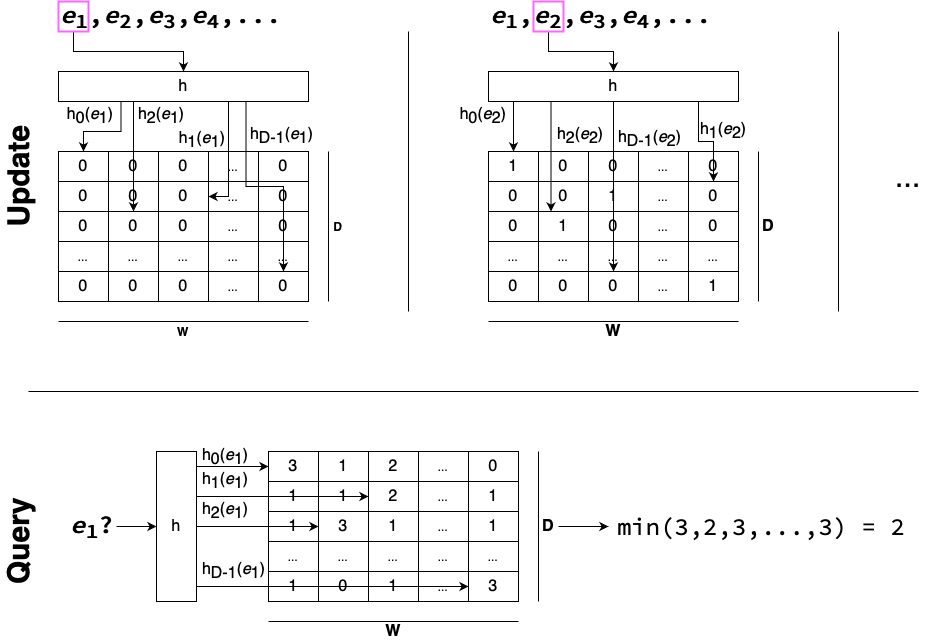
\includegraphics[width=0.9\textwidth]{figures/cm-example}
	\end{center}
	\caption{Example of a \cm sketch}\label{fig:countminexample}
\paguso{A ideia da figura está boa, mas precisa aumentar a fonte pra não ficar ilegível. Se não couber, simplifica a parte do incremento. Muda o label de Increment para Update.}
\end{figure}

It is important to notice that the \cm might overestimate the frequency of an event due to hash collisions, since more than one event might be mapped to the same cell of the matrix. However, the pairwise independence requirement ensures that, for any row $i$ and any two distinct events $e\neq e'$,
\begin{equation*}
\prob[h_i(e)=h_i(e')] = \frac{1}{W},
\end{equation*}
with this probability being computed over all possible choices of the hash function.
Hence, by setting $W$ appropriately, we can control the expected number of collisions per row, and likewise, by choosing a sufficiently large $D$, we can control for the probability of having at least one row without collisions for a given event. In general, for two given parameters $\epsilon, \delta \in (0,1)$, by setting 
$W=\frac{2}{\epsilon}$ and $D=\log\frac{1}{\delta}$, we have
\begin{equation}
\label{eq:cm-prob}
\prob[C.\mathit{query}(e) - f(e) > \epsilon F] < \delta,
\end{equation}
where $f(e)$ represents the true frequency of $e$, and $F=\sum_{e_i}f(e_i)$ is the true total event count. Put another way, we can have the estimate error relative to the total event count to be `small' (no more than $\epsilon$) with `good' (at least $1-\delta$) probability.

\subsection{Counting \kmer{s}}
\label{subsec:cm-countingkmers}

Zhang \emph{et al.} proposed using a \cm sketch to count \kmer{s} \cite{Zhang2014}. Each \kmer is treated as an event, with reads being processed as a stream of \kmer{s}. The \kmer{s} can be hashed by interpreting them not as a string, but as a base-4 integer, with $\A=0$, $\C=1$, $\G=2$, $\T=3$ (for example, the \kmer $\C\G\A\T\A$ can be interpreted as the integer $12030_4 = 396_{10}$). Whenever we refer to hashing a \kmer, we use its integer interpretation. This introduces the chance that any reported count will be an overestimate, the probability of which is approximately $(1-e^{-\frac{N}{W}})^D$, with $N$ the number of distinct \kmer{s} \cite{Zhang2014}.

\subsubsection{\cm as a probabilistic MDS representation for \dBG{s}}
\label{subsubsec:cm-dbg}

Because the \kmer counts are used to determine if a \kmer should be added to the \dBG, as discussed in Section~\ref{subsec:dBG-selectingkmers}, a structure that can answer count queries can be extended to implement the membership query operation, with a \kmer $X$ being considered to be represented in the graph if $C.\mathit{query}(X) \geq t$. As the count returned by the \cm sketch can be overestimated by some error $\epsilon F$ with probability $\delta$ as established in Equation~\ref{eq:cm-prob}, we can arrive at an expression for the probability that a low-frequency \kmer will be considered to be a member of the \dBG by taking into account the fact that most low-frequency \kmer{s} appear only once or twice in the reads and making $\epsilon F = t$. Due to the relationships between $W$ and $\epsilon$, and $D$ and $\delta$, we can decide the necessary size of the \cm sketch to minimize the expected false positive rate. Working backwards, with $W$ and $D$ established we can also choose $t$.

\section{The \dB\cm sketch}
\label{sec:debruijncountmin}

% - Representation (what goes in each cell)
% - Operations:
%   - addOutEdge
%   - query 
% - Analysis space/time (may be done within previous sections)

% Because we expect each \kmer from the sequence to appear in the reads a number of times equals to the coverage, while spurious \kmer{s} will appear a low number of times \cite{Conway2011} \cite{Ghosh2019}, a structure used to count \kmer{s} (that implements the $\mathit{count}(x)$) can implement the membership query operation as $\mathit{memb}(x)=\mathit{count}(x) \geq t$. In this way, a \cm sketch can \toconsider{probabilistically} represent a \dBG with some false positive and false negative rates associated with the membership query operation. These rates can be controlled by $t$.\asq{Aqui talvez valha a pena falar que existem duas abordagens para tentar controlar as taxas de falsos positivos e negativos: 1. O valor de $t$ pode ser estabelecido, e, então, os valores de $W$ e $D$ são calculados de forma a minimizar a chance de um erro $\epsilon > t$; 2. Os valores $W$ e $D$ podem ser fixados, e, então, $t$ é decidido baseado nas estimativas esperadas para um \kmer espúrio \emph{vs.} um \kmer real.}

% Selecting the appropriate value for $t$ is not a trivial task, however, and is a trade-off between the false positive and false negative rates. Due to the fact that reads are generated randomly from the original genome, and that a number of real \kmer{s} will be replaced by spurious \kmer{s} because of sequencing errors, an universally optimal threshold \toconsider{that perfectly decides if a \kmer is spurious or not} does not exist. Higher values of $t$ are more likely to cut out spurious \kmer{s}, reducing false positive rates, but they also increase the chances of a real \kmer being missed, increasing false negative rates. Lower values of $t$ result in the opposite effect happening.

In order to leverage the benefits of an NDS in reducing the impact of the false positive rate of the membership operation, we introduce a modified version of the \cm sketch, called \keyterm{\dB\cm} (\dBCM) allowing for querying not only for \kmer counts, but also for the outedges from the corresponding nodes in the \dBG. As such, the \dBCM implements not only the membership query operation as detailed in Section~\ref{subsubsec:cm-dbg}, but also a neighborhood query.


To store the additional information, we expand the \cm sketch such that each cell $C[i,j]$ in the matrix stores not only the counter $C[i,j].c$, but also a set of out-edges $C[i,j].E$. The structure then provides an operation to \emph{update} the counters $C[i,h_i(x)].C$ associated with a given \kmer $x$ by one, and an operation to \emph{add an out-edge} to the sets $C[i,h_i(x)].E$. The update operation is the same as in a regular \cm, and the procedure for adding an edge can be seen in Algorithm~\ref{alg:addOutEdge}.


\begin{algorithm}[htbp]
    \caption{$C.\mathit{add\_outedge}(X, a)$}\label{alg:addOutEdge}
    \Input{C, the \dBCM; $X$, the \kmer; $a \in \{\A, \C, \G, \T\}$, the outedge label}
    \For{$i \gets 0, \ldots, D-1$}{
      $C[i,h_i(X)].E \gets C[i,h_i(X)].E \cup \{a\}$\\
    }
\end{algorithm}

Furthermore, the \dBCM must accommodate this new information in its query operation. The sketch now returns not only the minimum value of the counters, but also the intersection of the sets of out-edges, as shown in in Algorithm~\ref{alg:query}.

\begin{algorithm}
	\caption{$C.\mathit{query}(X)$}\label{alg:query}
  \Input{$C$, the \dBCM; $X$, the \kmer}
  \Output{The estimated count $C$ and outedge set $E$}
	$c \gets \mathit{inf}$\\
	$E \gets \{\A, \C, \G, \T\}$\\
	\For{$i = 1, \ldots, D$}{
		$c \gets \min(c, C[i,h_i(X)].c)$\\
		$E \gets E \cap C[i,h_i(X)].E$\\
	}
	\Return{$(c, E)$}
\end{algorithm}

From a practical perspective, due to a node having at most four outedges corresponding to the bases $\{\A, \C, \G, \T\}$, the set storing them can be represented with four bits indicating whether each of them is present. An edge is added by setting the corresponding bit, and the intersection is obtained by performing the bitwise AND operation. Moreover the set of outedges and the counter are packed together in a single 16-bit integer. This layout can be visualized in Figure~\ref{fig:dbcm-bit_use}. When using a $k$ such that $4^k > |S|$, the each \kmer in $S$ is expected to appear only once. As such, it is expected to appear a number of times equals to the coverage $c$ in the reads. Considering that $c$ is not a very high value (commonly below $200$ \asq{Citation Needed?}), each counter can be represented by a 12-bit integer, accounting for the expected count for all real \kmer{s}, as well as any possible collisions.

\begin{figure}[htbp]
  \centering
  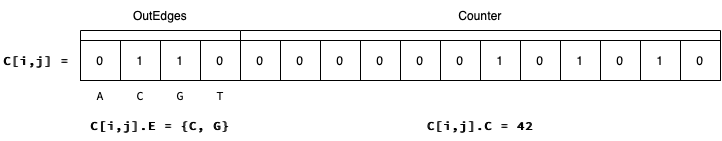
\includegraphics[width=0.9\textwidth]{figures/dbcm-bit_use}
  \caption{A cell from the \dBCM}\label{fig:dbcm-bit_use}
\end{figure}

\subsection{Using the \dBCM}

\subsubsection{Construction}

The \dBCM is constructed as the reads are processed by incrementing the counters for each \kmer as they are read. Once a \kmer{'s} counter reaches the threshold for presence $t$, an outedge is added from the \kmer that preceded it to itself. I.e. if \kmer{s} $X$ and $Y$ happen consecutively in a read, and $C.\mathit{query}(Y).C \geq t$, then the operation $C.\mathit{add\_outedge}(X, Y[k-1])$ is performed. A few things merit discussion:

\paragraph{There is no insert operation} Because the \dBCM is meant to be constructed straight from the reads, counting and filtering \kmer{s} during construction, there is no direct way to insert a \kmer in the graph. Instead, the \kmer{'s} count is incremented and it is only considered present once the count reaches or surpasses the threshold $t$.

\paragraph{The target node of an edge must exist before the edge is added, but not the source node} By only adding the edge $X\stackrel{a}{\longrightarrow}Y$ when $Y$ is considered to be high-frequency we avoid adding edges to nodes that we do not yet know to exist. Such edges would point, in the best case, to a node that would not be found to be on the graph, resulting in unnecessary operations before the path is considered finished, and in the worst case would be interpreted, in a collision, as a diferent edge, resulting in a new branch on the graph. Conversely, the source node $X$ does not need to be considered present on the graph for the edge to be added. This avoids the scenario where both $X$ and $Y$ are real \kmer{s}, but $Y$ shows up for the last time before $X$ is considered to be present, in which case the edge would never be added. Moreover, adding an outedge to a \kmer that is not considered to be present in the graph is irrelevant, as the \kmer will be ignored during traversal.

\subsubsection{Operations}

We can implement the operations listed in Section~\ref{subsubsec:dbg-operations} using the \dBCM operations as follows:

\paragraph{Membership query} Given the desired presence threshold $t$, we can implement the membership query operation in the \dBCM as $C.\mathit{is\_member}(X, t) = C.\mathit{query}(X).c \geq t$.\asq{I think it may be better to say that $t$ is a parameter of the \dBCM so that we don't need to pass it as an argument. And it makes sense, since the threshold is relevant during construction and would be weird to allow, for instance, of two different thresholds to be used (?)}
\paragraph{Forward neighbor query} $C.\mathit{forward\_neighbor}(X, a) = \{a\} \subseteq C.\mathit{query}(X).E$.
\paragraph{Neighborhood query} We can transform the set of outedges $C[i,j].E$ into a set of \kmer{s} by extending the \kmer with the outedges from the set. As such, a procedure for generating the set of neighbors for a given \kmer $X$ is found in Algorithm~\ref{alg:dbcm-neighbors}.

\begin{algorithm}
	\caption{$C.\mathit{neighbors}(X)$}\label{alg:dbcm-neighbors}
  \Input{$C$, the \dBCM; $X$, a \kmer}
  \Output{$N$, a set of \kmer{s} that are neighbors of $X$}
  $N \gets \emptyset$\\
  \For{$a \in C.\mathit{query}(X).E$}{
    $N \gets N \cup \{X[1:k-1] \cdot a\}$\\
  }
	\Return{$N$}
\end{algorithm}

\subsubsection{Navigation}

This structure can be navigated from an initial set of \kmer{s} by querying for their out-edges and then querying each of their neighbors, repeating this for each neighbor found to be in the graph. This procedure can be observed in Algorithm~\ref{alg:traversal}.

% \begin{algorithm}
% 	\caption{$C.\mathit{traverse}(\strsetname{S}, t)$}\label{alg:traversal}
%   \Input{$C$, the \dBCM; $\strsetname{S}$, the set of starting \kmer{s}; $t$, the threshold of presence}
%   \Output{$V$, the set of \kmer{s} queried from the \dBCM during traversal}
%   $F \gets$ empty Queue\\
%   \For{$s \in \strsetname{S}$}{
%     enqueue($F$, $s$)\\
%   }
%   $V \gets \{\}$\\
%   \While{$F$ is not empty} {
%     $u \gets$ dequeue($F$)\\
%     $V \gets V \cup \{u\}$\\
%     $n, E \gets C.query(u)$\\
%     \If{$n \geq t$}{
%       \For{$a \in E$}{
%         $v \gets$ extend($u$, $a$)\\
%         \If{$v \notin V$}{
%           enqueue($F$, $v$)\\
%         }
%       }
%     }
%   }
% 	\Return{$V$}
% \end{algorithm}

\begin{algorithm}
	\caption{$C.\mathit{traverse}(\strsetname{S}, t)$}\label{alg:traversal}
  \Input{$C$, the \dBCM; $\strsetname{S}$, the set of starting \kmer{s}; $t$, the threshold of presence}
  \Output{$V$, the set of \kmer{s} queried from the \dBCM during traversal}
  $F \gets$ empty Queue\\
  \For{$s \in \strsetname{S}$}{
    enqueue($F$, $s$)\\
  }
  $Q \gets \{\}$\\
  \While{$F$ is not empty} {
    $u \gets$ dequeue($F$)\\
    $Q \gets Q \cup \{u\}$\\
    \If{$C.\mathit{is\_member}(u, t)$}{
      \For{$v \in C.\mathit{neighbors}(u)$}{
        \If{$v \notin Q$}{
          enqueue($F$, $v$)\\
        }
      }
    }
  }
	\Return{$Q$}
\end{algorithm}

\paragraph{Selecting the starting set $\strsetname{S}$ of \kmer{s} for traversal} Ideally, only the first \kmer from the original sequence is needed to perform the traversal of the graph. It isn't possible to determine, however, where in the original sequence a read was taken from. One option is to use all the \kmer{s} from the reads that are found to be in the graph. This set can be constructed during construction of the \dBCM by evaluating if a newly incremented \kmer{'s} count surpasses the established threshold. This would create an unnecessarily large set, however: \toconsider{For \kmer{s} $X$ and $Y$ found in the same read such that $X$ precedes $Y$, we expect $Y$ to be reachable from $X$ and, threfore, adding $Y$ to \strsetname{S} is redundant.} We can, therefore, reduce the size of $\strsetname{S}$ by only considering the \kmer{s} that are at the start of their reads. To avoid the case where the first \kmer in each read is erroneous, we can take the first $n$ \kmer{s} from each read. \toconsider{In practice, however, this proved to be unnecessary, with $n=1$ still allowing for the complete traversal of the graph.}

\section{A space-efficiente Hashtable representation for \dBG{s}}
\label{sec:debruijnhashtable}
% - Structure
%   - fingerprint
%   - Outedges
% - Hash function 
% - Collision resolution
% - Operations 
%   - Add node/edge
%   - Query node/edge/star 
% - Analysis 

We also propose a new hashtable-based representation for the \dBG, called \dBHT (for \emph{\dB Hashtable}), that is made more space-efficient by not storing the \kmer directly. Instead, the slot $T[i]$ containing the \kmer $X$ stores a \keyterm{fingerprint} $T[i].f = f_X$, computed from $X$ as described in Section~\ref{sec:fingerprint}, along with the set of outgoing edges from $X$, $T[i].E$,  as described in Section~\ref{sec:debruijncountmin}.

When inserting a \kmer $X$ into the hashtable, a hash value $h_X$ and the fingerprint $f_X$ are calculated in parallel. The hash value, computed as described in Section~\ref{sec:fibhash}, determines the initial position $p_0$ in which the \kmer should be stored. If this slot is empty, then the fingerprint is written there. Otherwise, collisions are resolved by linear probing, that is the subsequent positions $(p_0+j)\mod m$, for $j=0\ldots m-1$, are checked until a free slot is found. If, however, a slot containing $f_X$ is found before, then $X$ is considered to be already represented in $H$ and the insertion aborts. This process is detailed in Algorithm~\ref{alg:ht-insert}. It makes sense to define the size of the hashtable, $m$, in terms of the number of distinct \kmer{s} $n$ that will occupy it and a \keyterm{load factor} $\alpha \in \mathbb{R}$ such that $m = \frac{n}{\alpha}$\asq{maybe use something other than $n$}. Higher values of $\alpha$ will result in a smaller and more space-efficient hashtable, but have a higher likelyhood of collisions occuring. Lower values present the opposite effect. Because we want the table to be able to store all distinct \kmer{s}, we're interested in $\alpha \leq 1$. Furthermore, because we depend on finding an empty position in order to determine that a \kmer is not present in the graph, as detailed below, we must also exclude $\alpha = 1$.

\begin{algorithm}
	\caption{$T.\mathit{insert}(X$)}\label{alg:ht-insert}
	\Input{$T$: a \dBHT with capacity $m$; $X$: the \kmer to be inserted}
	$h_X \gets \mathit{fibhash}(X, m)$\Comment{see Section~\ref{sec:fibhash}}\\
	$f_X \gets \mathit{fingerprint}(X)$\Comment{see Section~\ref{sec:fingerprint}}\\
	$i \gets h_X$\\
	\While{$T[i]$ is not empty}{
		\eIf{$T[i].f = f_X$}{
			\Return{}\Comment{$X$ already in $T$}
		}{
			$i \gets (i + 1)\mod m$\\
		}
	}
	$T[i].f\gets f_X$\\
	$T[i].E\gets \varnothing$\\
\end{algorithm}

To query the hashtable for a \kmer/node $X$, the same sequence of positions as in the insertion are probed until the desired fingerprint $f_X$ is found, or a free position is reached, in which case we can conclude that the \kmer is absent from the structure. This operation is presented in Algorithm \ref{alg:ht-query}.

\begin{algorithm}
	\caption{$T.\mathit{query}(X)$}\label{alg:ht-query}
  \Input{$T$: a \dBHT with capacity $m$; $X$: the \kmer to be queried}
	$h_X \gets \mathit{fibhash}(X, m)$\\
  $f_X \gets \mathit{fingerprint}(X)$\\
	$i \gets h_X$\\
	\While{$T[i]$ is not empty}{
    \eIf{$T[i].f = f_X$}{
      \Return{$T[i].E$}
    }{
		  $i \gets (i + 1) \mod m$\\
    }
	}
  \Return{$\varnothing$}
\end{algorithm}


Adding an edge $X\stackrel{a}{\longrightarrow}Y$ to the \dBHT is similar to adding a \kmer node, and breaks down to, first, locating the slot $T[i]$ of the source node $X$, and then adding the corresponding edge label $a$ to its set of outedges. As before, this is done by setting the appropriate bit of the  4-bit pattern $T[i].E$. The \dBHT does not verify that an edge being added targets a node already present in the graph. This is done because this verification happens naturally when inserting the \kmer{s} sequentially from the reads (given \kmer{s} $X$ and $Y$ consecutive in a read, $X$ is inserted before $Y$, but the edge $X\stackrel{a}{\longrightarrow}Y$ is only inserted when $Y$ is inserted), and also in the pipeline we present, where \kmer{s} and edges are obtained by traversing the \dBCM representation of the graph.\asq{Implementar essa verificação só pra retirar essa parte. Na verdade, dá pra modificar a inserção para verificar se as extensões do \kmer inserido estão contidos no grafo e aí adicionar as arestas relevantes, pra n precisar colocar as outedges separadamente} \toconsider{Querying such an edge then naturally consists in accessing that same position and checking $T[i].E$ to see if the corresponding bit is set.}\asq{Is this necessary? The query operation already returns all the outedges, so querying a specific edge can be as such: $T.\mathit{query\_edge}(X, a) = a \in T.\mathit{query}(X)$}


\begin{algorithm}
  \caption{$T.\mathit{add\_outedge}(X, a)$}\label{alg:ht-addedge}
  \Input{$T$: a \dBHT with capacity $m$; $X \in \{\A, \C, \G, \T\}^k$: the \kmer to be queried; $a \in \{\A, \C, \G, \T\}$: the edge label to be added}
  $h_X \gets \mathit{fibhash}(X, m)$\\
  $f_X \gets \mathit{fingerprint}(X)$\\
  $i \gets h_X$\\
  \While{$T[i]$ is not empty}{
    \eIf{$T[i].f = f_X$}{
      \Return{$a \in T[i].E$}
    }{
      $i \gets (i + 1) \mod m$\\
    }
  }
  \Return{$\varnothing$}
\end{algorithm}


\subsection{Modular Fibonacci Hashing}\label{sec:fibhash}

\asq{I need to revisit this because I need to make it make more sense}

\paguso{Na seção anterior, vc disse que o hash value e o fingerprint eram calculados simultaneamente. Nessas duas últimas seções, vc precisaria ter explicado isso melhor.
	O que acontece é o seguinte:
	Na realidade, primeiro vc identifica o kmer $X$ com um valor numérico de 64 bits considerando-o como um número de $k$ dígitos em base 4 com A=0 C=1 G=2 T=3. Isso você não mencionou.
	Em seguida vc aplica uma função de hashing não-criptográfica que é a tal fibonacci hashing $fibhash: 64bits \rightarrow 64bits$. O hash value de $X$ é o valor de $h(X)=fibhash(X)=1140\cdots85\cdot X\mod 2^{64}$. O módulo é implícito pela precisão do número 64 bits.
	Na prática vc acredita que $h(X)$ é um padrão de bits razoavelmente aleatórios e independentes entre si, e então vc usa esse hash value para simultaneamente extrair a posição e o fingerprint. Vc precisa contar a história dese jeito.
}

The \kmer is hashed using the Fibonacci hashing algorithm \cite{}, which leverages the property of the golden ratio $\phi$ that, given a range $r$, the set $\{(i \times \frac{r}{\phi} \mod r) | i \in \mathbb{N}\}$ is evenly distributed over $r$, and never repeats. The integer hashing algorithm that maps a number to the range $[0, m]$ works by multiplying the key $X$ by the closest integer to the value $\frac{m}{\phi}$ and returning the result modulo $m$. The $\mathit{fibhash}$ function can be seen in Algorithm~\ref{alg:fibonacci-hash}.
\paguso{É preciso explicar um pouco o algoritmo, não os detalhes, mas pelo menos o que está acontecendo. Tipo: a função mapeia um no. de 64bits noutro número de 64bits. Isso é feito multiplicando por uma constante grande $\phi=11400\cdots$ (dê um nome para evitar ficar usando essa constante literalmente). O resultado disso é que o valor resultante fica assim e assado, por isso e por isso. Uma análise experimental [citação] demonstra que os valores resultantes apresentam um bom efeito avalanche, ou seja, ao mudar um bit na entrada, cada bit da saída muda com 50\% de probabilidade. Do jeito que está, tá muito caído do céu isso.}

\begin{algorithm}
  \caption{$\mathit{fibhash}(X, m)$}\label{alg:fibonacci-hash}
  \Input{$X$, the key to be hashed; $m$, the range into which it should be hashed}
  \Return{$(\mathit{round}(\frac{m}{\phi}) \times X) \mod m$}
\end{algorithm}

\subsection{Fingerprint}\label{sec:fingerprint}

We obtain a 3-bit fingerprint by performing a modified version of the Fibonacci hashing algorithm: We use the hashing function described above for the range addressable by a 64-bit integer. Because the multiplication result will overflow, we can skip the modulo operation as it is performed implicitly. Then we take the three most significant bits of the result as the fingerprint.\asq{Why the most significant bits? Maybe because of the avalanche results?}

In practice this fingerprint function is very computationally efficient due to it foregoing the modulo operation and using a bitwise shift operation to extract the most significant bits. The result can be seen in Algorithm~\ref{alg:fingerprint}.

\begin{algorithm}
  \caption{$\mathit{fingerprint(X)}$}\label{alg:fingerprint}
  \Input{$X$, the key to fingerprint}
  \Return{$(X \times \mathit{round}(\frac{2^64}{\phi})) >> 61$}
\end{algorithm}

\subsection{Using the \dBHT}

\subsubsection{Construction}
\label{sec:dbht-construction}

We construct the \dBHT by traversing the \dBCM representation of the graph. Starting from a set of nodes, we insert the nodes into the \dBHT, we then insert all of its true neighbors, adding the corresponding outedges. Then the process is repeated for from those neighbors. This procedure can be seen in Algorithm~\ref{alg:ht-constructfromdbcm}.

\subsubsection{Operations}

\paragraph{Membership query} The membership query is just the evaluation of if the query operation found the \kmer: $T.\mathit{is\_member}(X) = T.\mathit{query}(X) \neq \varnothing$.

\paragraph{Forward neighbor query} As in the \dBCM, the forward neighbor query just checks if the given base $a$ is in the set of outedges of $X$: $T.\mathit{forward_neighbor}(X, a) = \{a\} \subseteq T.\mathit{query}(X)$.

\paragraph{Neighborhood query} Again like the \dBCM, the neighbors of $X$ can be obtained by extending it with its outedges, as presented in Algorithm~\ref{alg:dbht-neighbors}.

\begin{algorithm}
	\caption{$T.\mathit{neighbors}(X)$}\label{alg:dbht-neighbors}
  \Input{$T$, the \dBHT; $X$, a \kmer}
  \Output{$N$, a set of \kmer{s} that are neighbors of $X$}
  $N \gets \emptyset$\\
  \For{$a \in T.\mathit{query}(X)$}{
    $N \gets N \cup \{X[1:k-1] \cdot a\}$\\
  }
	\Return{$N$}
\end{algorithm}

\subsubsection{Navigation}

We navigate the \dBHT from a starting set of \kmer{s} \strsetname{S} by adding them to a queue. Then we dequeue one node and query for its neighbors, adding them to the queue if they weren't visited yet. We repeat this process until the queue is empty. This procedure can be seen in Algorithm~\ref{alg:dbht-navigate}. As in the traversal of the \dBCM, the result is the set of \kmer{s} that were queried during traversal.


\section{A pipeline using the \dBCM and the \dBHT}

Beyond the two isolated datastructures to represent the \dBG, we also propose a way to use both of them in tandem in order to obtain
the benefits of both. In this pipeline, the sequencing reads are processed and inserted into the \dBCM as they are made available,
such that the \dBG can be constructed online. Once the reads are all processed in this manner, and a navigatable version of the graph 
has been constructed, it can be traversed, with all of its nodes being, then, inserted in a \dBHT. In this way, a \dBCM is effectively
compressed into a \dBHT. This pipeline is formalized in Algorithm \ref{alg:pipeline}.
\paguso{O gap entre o que está descrito no texto e o Algoritmo está muito grande. Vc está deixando muito trabalho para o leitor descobrir o que está acontecendo através da leitura do Algoritmo. É preciso mostrar o Algoritmo e explicar o que está acontecendo. Por exemplo, precisa explicar a coisa dos complementos reversos, que nós/arestas estão sendo inseridos no \dBCM? O algoritmo tem um threshold $T$, mas de onde isso vem? Depois vc fala que o grafo pode ser percorrido. Como? Onde estão os nós âncora usados p/ percorrer o grafo? 
Há muitos detalhes importantes que não foram explicado aqui. Vc precisa fazer uma explicação topdown, colocar um diagrama. Por fim, esse algoritmo não é o que fazemos, não é? Por exemplo o threshold só é usado no percurso do grafo para decidir se é o nó real ou não, não durante a leitura das reads. Realmente, esta Seção está ruim e precisa ser totalmente refeita.}

\section{Experiments}

\subsection{Metrics}

\asq{Is accuracy the best term here? Why not precision, for example? Is there a more suitable term?}

\subsubsection{Representation Accuracy of the \dBCM}

The \dBCM has two aims: (1) counting the \kmer{s} from the reads, and (2) implementing a navigatable representation of a \dBG. Due to its probabilistic nature, however, it cannot achieve deterministic exactness in either of those aims. It becomes important, therefore, to evaluate how accurate it is at each of them. To do so, we compare its estimated count for each of the \kmer{s} in the reads to the \kmer{s} actual count. We also test the false positive and false negative rates of the sketch before traversal.

\paragraph{Count Accuracy} To evaluate count accuracy, distribution of estimated counts agains that of actual counts. We also look at the mean and standard deviation of the count errors $\{C.query(X).c - f(X) | X \in \readset\}$. Because the \cm sketch will only err by overestimation, the error is always a positive value, and therefore we can take its mean directly instead of using something like the mean squared error.

\paragraph{False Positives} When evaluating the accuracy of the \dBCM, it makes sense to test how many of the spurious \kmer{s} present in \readset attained a count high enough to be considered represented in the graph. As such, we begin by defining the set of \kmer{s} from the sequence $K = \{X | X \in \strname{S}\}$ and the set of nodes of $G$ as $V = \{X | X \in \readset, C.\mathit{query}(X).c \geq t\}$. Then we obtain the set of false positives as $F_p = V \setminus K$ and define a false positive rate as $f_p = \frac{|F_p|}{|V|}$.

\paragraph{False Negatives} Similarly to false positives, we can look at the \kmer{s} from the original sequence that are not represented in the graph because they don't reach the threshold $t$. Again we define the sets $K$ and $V$. Then, we obtain the set of false negatives as $F_n = K \setminus V$, and the false negative rate as $f_n = \frac{|F_n|}{|K|}$.

\subsubsection{Graph Traversal}

By implementing the \dBCM and \dBHT as navigational structures, however, we aim at reducing the impact of false positives as defined above by only querying for neighbors of known members. In this way, a false positive \kmer might never be queried if its in-neighbors are considered to not be represented in the graph. In this way, a true negative can stop a false positive from happening down the path. Conversely, a false negative can theoretically cause a true positive to never be queried, ultimately causing it to become a false negative as well.

We change the definitions of false positives and false negatives by changing the definition of the set of nodes of $G$ to be the set of nodes \emph{visited during traversal} of $G$: $V = \{X | X \in B.\mathit{traverse}(\strsetname{S}), B.\mathit{is\_member}(X)\}$. Then, as above, we have $F_p = V \setminus K$ and $f_p = \frac{|F_p|}{|V|}$, and $F_n = K \setminus V$ and $f_n = \frac{|F_n|}{|K|}$.

\subsection{\emph{E.~Coli}}

We use the \emph{E.~Coli} genome \cite{} as a benchmark through three different experiments. Firstly, we take the reference genome and generate a read set \readset without sequencing errors or reverse complements. Then, we add the presence of the reverse complements and, finally, we use the \emph{ART Illumina} toolkit \cite{Huang2011} to generate realistic reads from the genome, including sequencing errors and reverse complements.

Through all of these experiments, we processed the reads by adding their \kmer{s} in a \dBCM sketch, then repeating the process for its reverse complement. The \kmer{s} were then counted exactly through the use of a hashtable, and the counts were saved along with the estimated counts from the sketch. Finally, we traversed the sketch, saving all the queried \kmer{s} along with the query result. A \dBHT was constructed as described in Section~\ref{sec:dbht-construction}, and the resulting structure was traversed as well. With this we were able to analyse the metrics described above.

\subsubsection{Synthetic Reads without Errors and Reverse Complements}

Given the reference genome $S$, the length of each read, $L$, and the desired coverage $C$, the synthetic reads were generated by picking
$\frac{|S| \times C}{L}$ substrings of $S$ at random. This is presented in algorithmic form in Algorithm \ref{alg:generate-reads}.

\begin{algorithm}
  \caption{Generate Reads}\label{alg:generate-reads}
  \Input{$S$, the reference genome, $L$ the read length, $C$ the coverage}
  \Output{A set of reads $\readset$}
  $n \gets \frac{|S| \times C}{L}$\\
  $\readset \gets \emptyset$\\
  \For{$i \gets 1, \ldots, n$}{
    $j \gets \mathit{random}(0, |S| - L)$\\
    $\readset \gets \readset \cup \{S[j: j+L]\}$\\
  }
  \Return{$\readset$}
\end{algorithm}

\subsubsection{Synthetic Reads without Errors and with Reverse Complements}

The same procedure was used as in the previous section, but each individual read had a 50\% chance of being generated from the reverse complement of the reference genome \strname{S}

\subsubsection{Synthetic Reads with Errors}

In order to simulate the reads as they would be produced by the sequencing process, we used the ART Illumina toolkit to generate
synthetic reads from the \emph{E.~Coli} genome. The reads were generated using the following parameters:

\begin{enumerate}
\item \textbf{Sequencing System}: Illumina MiSeq v3
\item \textbf{Read length}: \textit{250bp}
\item \textbf{Coverage}: \textit{80x}
\end{enumerate}